% !TeX spellcheck = es_ES
\documentclass[12pt, titlepage]{article}
\usepackage[letterpaper, margin=2.5cm]{geometry}
% MATEMATICAS
\usepackage{amsmath}
% IDIOMA %
\usepackage[utf8]{inputenc}
\usepackage[spanish]{babel}
% IMAGENES
\usepackage{graphicx} 
\usepackage{float}
% COLORES
\usepackage{color}
\definecolor{dkgreen}{rgb}{0,0.6,0}
\definecolor{gray}{rgb}{0.5,0.5,0.5}
\definecolor{mauve}{RGB}{253,151,31}
\definecolor{deepred}{RGB}{249,38,114}
% CODIGO %
\usepackage{listings}
\lstset{
    frame=tb,
    language=Python,
    aboveskip=3mm,
    belowskip=3mm,
    showstringspaces=false,
    columns=flexible,
    numbers=left,
    stepnumber=1,
    basicstyle={\small\ttfamily},
    numberstyle=\tiny\color{gray},
    keywordstyle=\color{blue},
    commentstyle=\color{dkgreen},
    stringstyle=\color{mauve},
    breaklines=true,
    breakatwhitespace=true,
    tabsize=2,
    morekeywords={self, append, keys, len, get, TablaLL},
    emph={},
    emphstyle=\color{deepred}
}

%opening
\title{Reporte: Práctica 6}
\author{Barrera Pérez Carlos Tonatihu \\ Profesor: Saucedo Delgado Rafael 
Norman 
\\ Compiladores \\ Grupo: 3CM6}

\begin{document}
    \maketitle
    \tableofcontents
    \newpage
    \section{Introducción}
    Para la construcción de la tabla LL(1) es necesario el uso de dos métodos 
los cuales son \emph{PRIMERO} y \emph{SIGUIENTE}, estos dos métodos nos 
permiten elegir que producción se utilizara con base al símbolo de 
entrada. \cite{compis}

Estas dos operaciones se definen de la siguiente forma.
\begin{itemize}
    \item \emph{PRIMERO($\alpha$)}. Donde $\alpha$ es una cadena de símbolos 
gramaticales es el conjunto de terminales que empiezan la las cadenas derivadas 
a partir de $\alpha$.
    \item \emph{SIGUIENTE(A)}. Donde \emph{A} es un no terminal es el conjunto 
de terminales \emph{a} que pueden aparecer de inmediato a la derecha de 
\emph{A}.
\end{itemize}
Ahora bien, para calcular \emph{PRIMERO(X)} donde $X$ es un símbolo gramatical 
se aplican las siguientes reglas hasta que no puedan agregarse mas terminales o 
$\epsilon$.
\begin{itemize}
    \item Si $X$ es un terminal entonces \emph{PRIMERO(X)} = 
$\left\lbrace X \right\rbrace $.
    \item Si $X$ es un no terminal entonces por cada producción de $X$
    \[X \rightarrow Y_1 Y_2 Y_3\ldots Y_m\]
    \begin{itemize}
     \item Agregar \emph{PRIMERO($Y_i$)} a \emph{PRIMERO(X)}.
     \item Si \emph{PRIMERO($Y_i$)} contiene $\epsilon$ 
avanza $i$.
    \end{itemize}
\end{itemize}
Por otro lado para calcular \emph{SIGUIENTE(N)} se 
siguen las siguientes reglas.
\begin{itemize}
 \item Si $N$ es inicial. Agregar $\$$ a \emph{SIGUIENTE(N)}.
 \item Si $A \rightarrow \alpha N$. Agregar \emph{SIGUIENTE(A)}.
 \item Si $A \rightarrow \alpha N \beta$. Agregar \emph{PRIMERO($\beta$)}.
 \item Si $A \rightarrow \alpha N$ y $\epsilon \in $ \emph{PRIMERO($\beta$)}. 
Agregar \emph{SIGUIENTE(A)}.
\end{itemize}
\begin{figure}[H]
        \begin{center}
            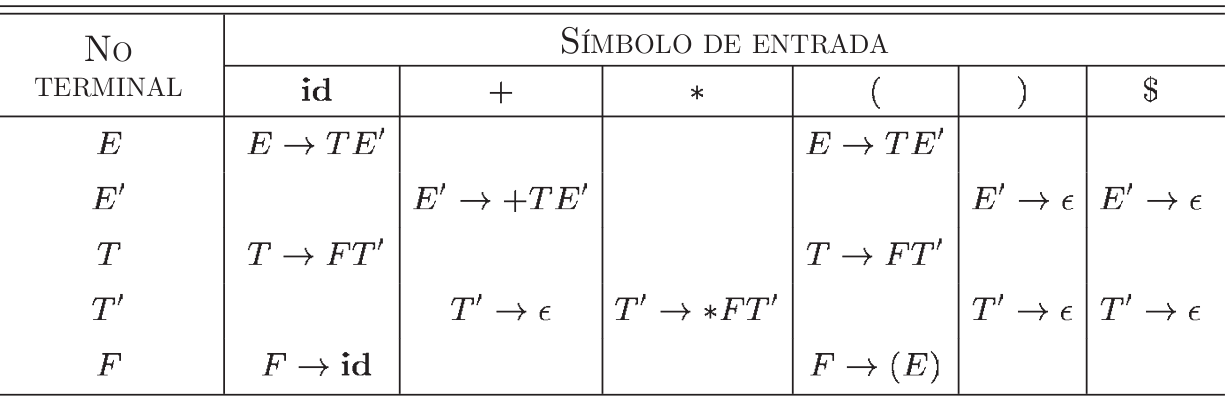
\includegraphics[width=15cm]{tabla.png}
            \caption{Tabla de análisis sintáctico M \cite{compis}.}
            \label{fig:tabla}
        \end{center}
\end{figure}
Ya que se tiene la definición de las funciones \emph{PRIMERO} y 
\emph{SIGUIENTE} se tiene que construir la tabla $M$ como la mostrada en la 
figura \ref{fig:tabla} para poder realizar el análisis sintáctico, esta creación 
se realiza utilizando el siguiente algoritmo. \cite{compis}
\begin{enumerate}
 \item Por cada producción $A \rightarrow \alpha$
 \begin{enumerate}
  \item Por cada $a$ en primero \emph{PRIMERO($\alpha$)}.
  \begin{enumerate}
   \item Agregar $A \rightarrow \alpha$ en $M\left[A, a \right] $.
  \end{enumerate}
  \item Si $\epsilon \in $ \emph{PRIMERO($\alpha$)}
  \begin{enumerate}
   \item Agregar $A \rightarrow \alpha$ en $M\left[A, c \right] $ para cada $c$ 
en \emph{SIGUIENTE(A)}.
  \end{enumerate}
 \end{enumerate}
\end{enumerate}
Un ejemplo de la construcción de esta tabla se encuentra en la figura 
\ref{fig:tabla} dicha tabla se construyo utilizando la siguiente gramática.
    \begin{align*}
        E &\rightarrow TE' \\
        E' &\rightarrow +TE' \mid \epsilon \\
        T &\rightarrow FT' \\
        T' &\rightarrow *FT' \mid \epsilon \\
        F &\rightarrow (E) \mid \text{\textbf{id}}\\
    \end{align*}
    \newpage
    \section{Desarrollo}
Para la creación de la tabla LL(1) se definieron tres clases para poder hacer 
uso de la herencia y con ello poder separar el código de una forma que sea más 
fácil de entender además de que permita la reutilización de este.

    Esta es una clase muy importante ya que facilita la manipulación de 
gramáticas ya que permite un acceso rápido a los componentes de una gramática 
libre de contexto.
    \begin{lstlisting}[title=Archivo: gramatica.py]
import re


class Gramatica:
    """Clase que almacena los componentes de una gramatica:
        - terminales
        - no terminales
        - producciones
        - simbolo inicial
        Tambien se encarga de leer la gramatica del archivo
        y almacenarla"""
    def __init__(self, archivo):
        self.nombre_archivo = archivo
        self.no_terminales = dict()
        self.terminales = dict()
        self.inicial = None
        self.gramatica = dict()

    def leer_archivo(self):
        """Metodo que lee el archivo y obtiene
        los componentes de la gramatica"""
        archivo = open(self.nombre_archivo, 'r')
        primera = 0
        j = 0
        for linea in archivo:
            if primera == 0:
                self.obtener_no_terminales(linea)
                primera = 1
                continue
            if primera == 1:
                self.inicial = linea[0]
                primera = 2
            j = self.obtener_produccion(linea, j)
        self.terminales.update({"$": j})

    def obtener_produccion(self, linea, j):
        """Metodo cada produccion"""
        izq = linea[0]
        der = linea[3:]
        der = re.match("[^\n]*", der).group()
        if izq not in self.gramatica:
            self.gramatica.update({izq: {
                "producciones": list(),
                "primero": False,
                "siguiente": False
            }})
        self.gramatica.get(izq).get("producciones").append(der)
        for c in der:
            busqueda = re.match("[a-df-z\(\)\+\-\*]", c) is not None
            if busqueda and c not in self.terminales:
                self.terminales.update({c: j})
                j += 1
        return j

    def obtener_no_terminales(self, linea):
        """Obtiene los terminales de la primera linea del archivo"""
        i = 0
        for c in linea:
            busqueda = re.match("[A-Z]", c) is not None
            if busqueda and c not in self.no_terminales:
                self.no_terminales.update({c: i})
                i += 1
    \end{lstlisting}
    Esta clase es donde están declaradas las funciones \emph{PRIMERO} y 
\emph{SIGUIENTE}. Hereda de clase \emph{Gramatica} para poder trabajar con 
alguna gramática y facilitar su manipulación.
    \begin{lstlisting}[title=Archivo: auxiliares.py]
from gramatica import Gramatica
import re


class Auxiliares(Gramatica):
    """Clase que contiene la implementacion de los
    metodos primero y siguiente"""
    def __init__(self, archivo):
        """Se envia el nombre del archivo
        a la clase padre"""
        super(Auxiliares, self).__init__(archivo)

    def es_epsilon(self, A):
        return A == 'e'

    def es_terminal(self, A):
        return A not in self.gramatica

    def es_inicial(self, S):
        return self.inicial == S

    def primero(self, A):
        """Metodo que calcula primero de una cadena"""
        conjunto = set()
        for a in A:
            if a in self.gramatica:
                self.gramatica.get(a)["primero"] = False
            conjunto_extra = self.P(a)
            conjunto.update(conjunto_extra)
            if 'e' not in conjunto_extra:
                if 'e' in conjunto:
                    conjunto.remove('e')
                break
        return conjunto

    def P(self, A):
        """Metodo que calcula primero de un solo simbolo"""
        conjunto = set()
        if self.es_terminal(A) or self.es_epsilon(A):
            conjunto.add(A)
        else:
            if self.gramatica.get(A).get("primero"):
                return conjunto
            else:
                self.gramatica.get(A)["primero"] = True

            producciones = self.gramatica.get(A).get("producciones")
            for produccion in producciones:
                i = 0
                while i < len(produccion):
                    extra = self.P(produccion[i])
                    conjunto.update(extra)
                    if 'e' in extra:
                        i += 1
                    else:
                        break
        return conjunto

    def siguiente(self, N):
        """Metodo para el calculo de siguiente
        se inicializan los banderas que indican si ya
        se calculo siguiente"""
        for clave, valor in self.gramatica.items():
            valor["siguiente"] = False
        return self.S(N)

    def S(self, N):
        """Calculo de siguiente"""
        conjunto = set()
        if not self.es_terminal(N) and self.gramatica.get(N).get("siguiente"):
            return conjunto
        else:
            if not self.es_terminal(N):
                self.gramatica.get(N)["siguiente"] = True

        if self.es_inicial(N):
            conjunto.add('$')
        # A -> xN
        no_terminales = self.obtener_izquierda(N)
        if len(no_terminales) != 0:
            for n in no_terminales:
                conjunto.update(self.S(n))
        # A -> xNy
        no_terminales = self.obtener_derecha(N)
        if len(no_terminales) != 0:
            for simbolo in no_terminales:
                primero = self.primero(simbolo.get("cadena"))
                if 'e' in primero:
                    primero.remove('e')
                    conjunto.update(self.S(simbolo.get("clave")))
                conjunto.update(primero)
        if not self.es_terminal(N):
            self.gramatica.get(N)["siguiente"] = False
        return conjunto

    def obtener_izquierda(self, N):
        """Obtiene la parte izquierda de una produccion"""
        claves = list()
        for clave, valor in self.gramatica.items():
            for v in valor.get("producciones"):
                if N == v[len(v)-1]:
                    claves.append(clave)
        return claves

    def obtener_derecha(self, N):
        """Obtiene la parte derecha de una produccion"""
        simbolos = list()
        for clave, valor in self.gramatica.items():
            for v in valor.get("producciones"):
                for m in re.finditer(N, v):
                    if m.start() != len(v)-1:
                        simbolos.append({
                            "clave": clave,
                            "cadena": v[m.start()+1:]
                            })
        return simbolos

    \end{lstlisting}
    Esta clase es la encargada de construir la tabla con el algoritmo antes 
mencionado, hereda de la clase Auxiliares para poder utilizar las funciones de 
\emph{PRIMERO} y \emph{SIGUIENTE}.
    \begin{lstlisting}[title=Archivo: tabla.py]
from auxiliares import Auxiliares


class TablaLL(Auxiliares):
    """Clase para la creacion y despliegue de la tabla LL(1)
    utilizando los metodos contenidos en la clase padre Auxiliares"""
    def __init__(self, archivo):
        """Se recibe el nombre del archivo y se pasa a la clase padres"""
        super(TablaLL, self).__init__(archivo)
        self.leer_archivo()
        self.num_filas = len(self.no_terminales)
        self.num_colum = len(self.terminales)
        self.tabla = [[None] * self.num_colum for i in range(self.num_filas)]

    def construir_tabla(self):
        """Implementacion del algoritmo para el
        llenado de la tabla"""
        produccion_num = 1
        for clave, valor in self.gramatica.items():
            for produccion in valor.get("producciones"):
                primeros = self.primero(produccion)
                for a in primeros:
                    if a != "e":
                        self.agregar_elemento(clave, a, produccion_num)
                if "e" in primeros:
                    siguientes = self.siguiente(clave)
                    for c in siguientes:
                        self.agregar_elemento(clave, c, produccion_num)

                produccion_num += 1

    def agregar_elemento(self, A, a, num):
        """Metodo que agrega un elemento a la tabla"""
        i = self.no_terminales.get(A)
        j = self.terminales.get(a)
        if self.tabla[i][j] is None:
            self.tabla[i][j] = set()
        self.tabla[i][j].add(num)

    def mostrar_tabla(self):
        """Metodo que muestra la tabla"""
        print("Tabla LL(1):")
        print("    ", end="")
        for t in self.terminales.keys():
            print(t, end="\t")
        print("")
        for f, n in zip(self.tabla, self.no_terminales.keys()):
            for c in f:
                print(c, end="\t")
            print(n)
    \end{lstlisting}
    Este archivo es en el cual se realizan las pruebas, después de ejecutarlo 
se introduce el nombre del archivo que contiene la gramática.
    \begin{lstlisting}[title=Archivo: prueba.py]
from tabla import TablaLL
# creacion de la tabla LL(1)
gramatica = input("Nombre del archivo: ")
tabla = TablaLL(gramatica)
tabla.construir_tabla()
tabla.mostrar_tabla()
    \end{lstlisting}


    \newpage
    \section{Resultados}
    Para comprobar que la creación de la tabla se realiza de forma correcta se 
realizaron 3 pruebas con gramáticas diferentes. Dichas gramáticas se ingresan 
mediante un archivo de texto que contiene dicha una gramática, además de tener 
la gramática el archivo tiene los símbolos no terminales en la primera linea 
del archivo.
    \subsection{Prueba 1}
    Gramática usada en esta prueba.
    \setcounter{equation}{0}
    \begin{align}
        S &\rightarrow abBCa \\
        B &\rightarrow bACA \\
        B &\rightarrow aC \\
        C &\rightarrow bAbS \\
        C &\rightarrow e \\
        A &\rightarrow a \\
        A &\rightarrow e
    \end{align}
    Salida del programa.
    \begin{figure}[H]
        \begin{center}
            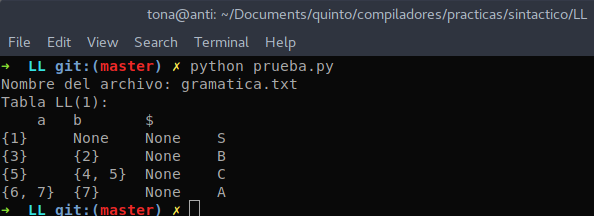
\includegraphics[width=15cm]{gramatica.png}
            \caption{Tabla LL(1).}
            \label{fig:prueba1}
        \end{center}
    \end{figure}
    Después de observar esta tabla podemos concluir que esta gramática 
produciría problemas debido a que hay más de un elemento en una celda de la 
tabla.
    \subsection{Prueba 2}
    Gramática usada en esta prueba.
    \setcounter{equation}{0}
    \begin{align}
        S &\rightarrow iEtSD \\
        S &\rightarrow a \\
        D &\rightarrow oS \\
        D &\rightarrow e \\
        E &\rightarrow b
    \end{align}
    Salida del programa.
    \begin{figure}[H]
        \begin{center}
            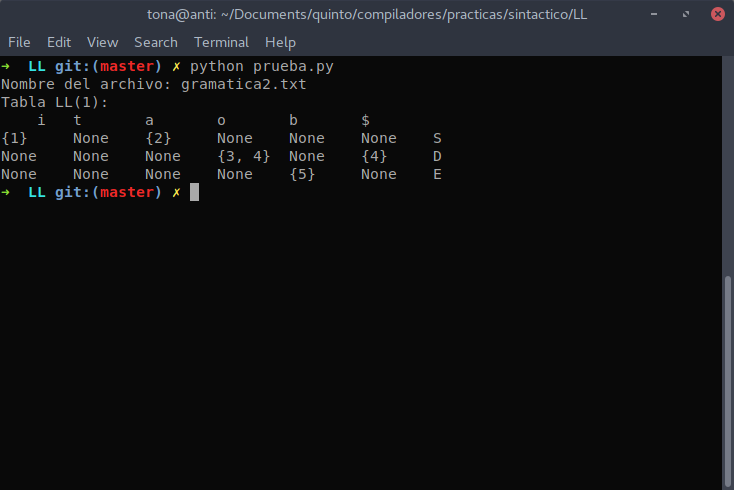
\includegraphics[width=15cm]{gramatica2.png}
            \caption{Tabla LL(1).}
            \label{fig:prueba2}
        \end{center}
    \end{figure}
    Después de observar esta tabla podemos concluir que esta gramática 
produciría problemas debido a que hay más de un elemento en una celda de la 
tabla.
    \subsection{Prueba 3}
    Gramática usada en esta prueba.
    \setcounter{equation}{0}
    \begin{align}
        E &\rightarrow TR \\
        R &\rightarrow +TR \\
        R &\rightarrow e \\
        T &\rightarrow FY \\
        Y &\rightarrow *FY \\
        Y &\rightarrow e \\
        F &\rightarrow (E) \\
        F &\rightarrow i
    \end{align}
    Salida del programa.
    \begin{figure}[H]
        \begin{center}
            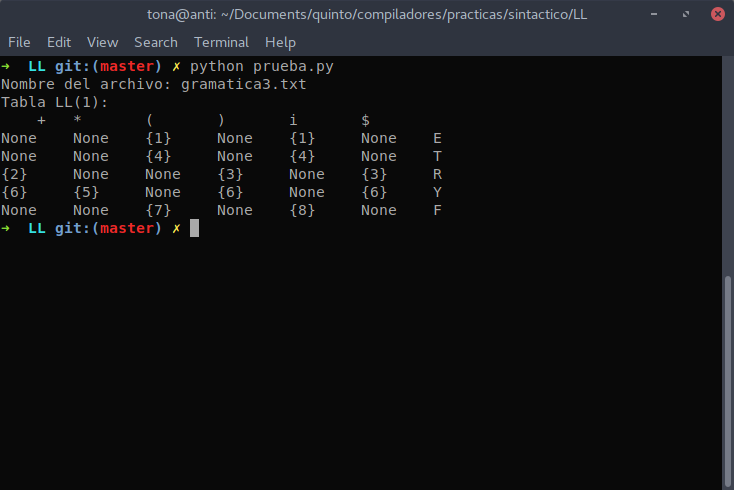
\includegraphics[width=15cm]{gramatica3.png}
            \caption{Tabla LL(1).}
            \label{fig:prueba3}
        \end{center}
    \end{figure}
    Esta tabla no produce ningún problema por lo que podría ser utilizada en el 
siguiente paso del análisis sintáctico.
    \newpage
    \section{Conclusiones}
    El uso de este tipo de analizadores resulta ser más poderosos que utilizar 
un analizador por descenso recursivo, sin embargo, aun existen problemas 
trabajando con gramáticas recursivas por la izquierda y con aquellas que pueden 
generar ambigüedades. Este es un serio problema debido a que a pesar de existir 
técnicas para eliminar la recursión por la izquierda no siempre es sencillo 
realizar este procedimiento por lo que al final optar por un tipo de analizador 
más poderoso puede reducir el tiempo de trabajo que se tenga que realizar.

Finalmente se puede concluir que de trabajar con alguna gramática sencilla 
utilizar este tipo de analizador seria lo indicado ya que no es difícil de 
entender ni de implementar.
    \bibliography{reporte} 
    \bibliographystyle{ieeetr}
\end{document}
